\documentclass[12pt,a4paper,bibliography=totocnumbered,listof=totocnumbered]{scrartcl}

\usepackage[english]{babel}
\usepackage[utf8]{inputenc}
\usepackage{amsmath}
\usepackage{amsfonts}
\usepackage{amssymb}
\usepackage{graphicx}
\usepackage{fancyhdr}
\usepackage{tabularx}
\usepackage{geometry}
\usepackage{setspace}
\usepackage[right]{eurosym}
\usepackage[printonlyused]{acronym}
\usepackage{subfig}
\usepackage{floatflt}
\usepackage[usenames,dvipsnames]{color}
\usepackage{colortbl}
\usepackage{color}
\usepackage{paralist}
\usepackage{array}
\usepackage{titlesec}
\usepackage{parskip}
\usepackage[right]{eurosym}
\usepackage[subfigure,titles]{tocloft}
\usepackage[pdfpagelabels=true]{hyperref}
\usepackage{units}
\usepackage{booktabs}
\usepackage{listings}
\usepackage{float}
\usepackage{bold-extra}
\lstset{mathescape=true,
        %frame=tB,
        numbers=left, 
        numberstyle=\tiny,
        basicstyle=\ttfamily\footnotesize, 
        numbers=left,
        morekeywords={Input, for, in},
        keywordstyle = \bfseries,
        xleftmargin=.04\textwidth, 
        captionpos=b,
        breaklines=true, 
        showstringspaces=false, 
        tabsize=2, 
        frame=shadowbox}
\renewcommand{\lstlistingname}{Algorithmus}% Listing -> Algorithm
\captionsetup[lstlisting]{font={small}}
\makeatletter
\def\l@lstlisting#1#2{\@dottedtocline{1}{0em}{1em}{\hspace{1,5em} Lst. #1}{#2}}
\makeatother

\geometry{a4paper, top=25mm, left=20mm, right=20mm, bottom=25mm, headsep=10mm, footskip=12mm}


\graphicspath{{../Figures/}}

\hypersetup{unicode=false, pdftoolbar=true, pdfmenubar=true, pdffitwindow=false, pdfstartview={FitH},
	pdftitle={Ausarbeitung Evolutionsstrategien als Alternative zu Bestärkendem Lernen im Bereich der Künstlichen Intelligenz},
	pdfauthor={Daniela Schacherer},
	pdfsubject={Seminararbeit},
	pdfcreator={\LaTeX\ with package \flqq hyperref\frqq},
	pdfproducer={pdfTeX \the\pdftexversion.\pdftexrevision},
	pdfkeywords={Seminararbeit},
	pdfnewwindow=true,
	colorlinks=true,linkcolor=black,citecolor=black,filecolor=magenta,urlcolor=black}
\pdfinfo{/CreationDate (D:20110620133321)}
\newcommand*{\source}{%
  \footnotesize Source:
  }

\begin{document}

\titlespacing{\section}{0pt}{12pt plus 4pt minus 2pt}{-6pt plus 2pt minus 2pt}

% Kopf- und Fusszeile
\renewcommand{\sectionmark}[1]{\markright{#1}}
\renewcommand{\leftmark}{\rightmark}
\pagestyle{fancy}
\lhead{}
\chead{}
\rhead{\thesection\space\contentsname}
\cfoot{}
\rfoot{\thepage}
\renewcommand{\headrulewidth}{0.4pt}
\renewcommand{\footrulewidth}{0.4pt}

% Vorspann
\renewcommand{\thesection}{\Roman{section}}
\renewcommand{\theHsection}{\Roman{section}}
\pagenumbering{Roman}

% %----------------------------------------------------------------------------------------
%	TITLE PAGE
%----------------------------------------------------------------------------------------

\begin{titlepage}

\newcommand{\HRule}{\rule{\linewidth}{0.5mm}} % Defines a new command for the horizontal lines, change thickness here

\center % Center everything on the page

\LARGE Ruprecht-Karls-University Heidelberg \\[0.5cm] % Name of your university/college
\Large Faculty of Mathematics and Computer Science \\[1.5cm]
\Large \textbf{Project}: Object Recognition and Image Understanding\\[0.5cm] % Major heading such as course name

\HRule \\[0.4cm]
{ \textsc{\huge \bfseries Traffic Sign Detection in Colour Images}}\\ \textsc{\Large two approaches in comparison}\\[0.4cm] % Title of your document
\HRule \\[1.5cm]

\begin{minipage}{0.4\textwidth}
\begin{flushleft} \large
\emph{Author:}\\
Daniela Schacherer, 3165890, M.Sc. Angewandte Informatik \\
Marvin Klaus, 3486809, M.Sc. Angewandte Informatik \\% Your name
\end{flushleft}

\begin{flushleft} \large
\emph{Lecturer:}\\
Prof. Björn Ommer \\ % Your name
\end{flushleft}

\begin{flushleft} \large
\emph{Date}\\
24.07.2018 \\% Your name
\end{flushleft}

\end{minipage}
~
\begin{minipage}{0.4\textwidth}
\end{minipage}\\[4cm]

\vfill % Fill the rest of the page with whitespace

\end{titlepage}

%----------------------------------------------------------------------------------------
%	INHALTSVERZEICHNIS
%----------------------------------------------------------------

\tableofcontents % Include a table of contents

\newpage % Begins the essay on a new page instead of on the same page as the table of contents 


% ----------------------------------------------------------------------------------------------------------
% Inhalt
% ----------------------------------------------------------------------------------------------------------
% Abstände Überschrift
\titlespacing{\section}{0pt}{12pt plus 4pt minus 2pt}{-6pt plus 2pt minus 2pt}
\titlespacing{\subsection}{0pt}{12pt plus 4pt minus 2pt}{-6pt plus 2pt minus 2pt}
\titlespacing{\subsubsection}{0pt}{12pt plus 4pt minus 2pt}{-6pt plus 2pt minus 2pt}

% Kopfzeile
\renewcommand{\sectionmark}[1]{\markright{#1}}
\renewcommand{\subsectionmark}[1]{}
\renewcommand{\subsubsectionmark}[1]{}
\lhead{Chapter \thesection}
\rhead{\rightmark}

\onehalfspacing
\renewcommand{\thesection}{\arabic{section}}
\renewcommand{\theHsection}{\arabic{section}}
\setcounter{section}{0}
\pagenumbering{arabic}
\setcounter{page}{1}


\section{Introduction}
Autonomous driving is nowadays one of the most growing research fields. In this context visual detection and recognition of road signs becomes particularly important. The project presented in this report aims at the exploration of two state-of-the-art approaches towards the detection of traffic signs in color images. In contrast to traffic sign recognition, detection aims merely at locating the traffic signs in the images, however, not at classifying them. 

\section{Dataset}
The dataset employed for this task was made publicly available by the University of Bochum as part of a traffic sign detection competition in 2013 \cite{dataset}. The data set comprises 900 images (1360 $\times$ 800 pixels) in PPM format containing 1206 traffic signs. Additionally, the image sections containing only the traffic signs and a CSV file containing ground truth information (location of the traffic signs within the images) are provided. Each image contains zero to six of those traffic signs included in the competition like, for example, speed limit or stop signs. For a complete list of the competition relevant categories see Appendix A. The sizes of the traffic signs in the images vary from $16$ to $128$ pixels w.r.t the longer edge \cite{Houben-IJCNN-2013}. \\
The images were collected such that different street scenes as urban, rural, or highway as well as different lightning and weather conditions  are equally represented in the dataset. Figure \ref{fig:ex_images} shows some examples contained in the data set. \cite{Houben-IJCNN-2013}.
\begin{figure}[H]
  \centering
  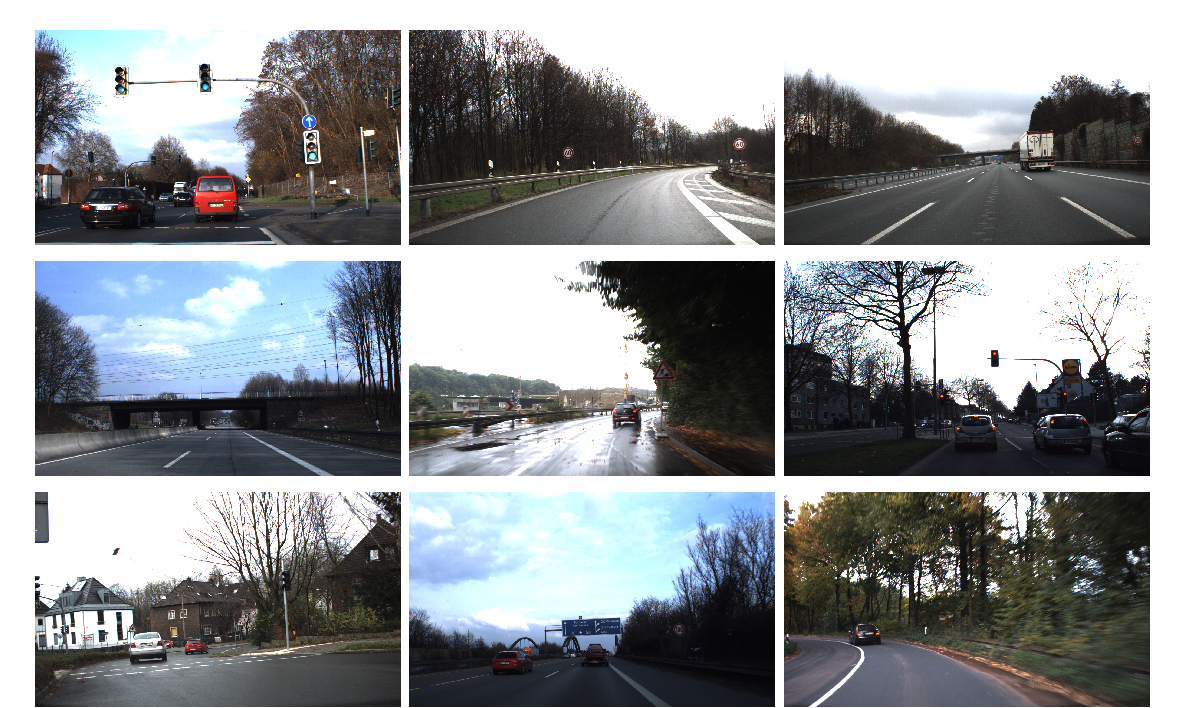
\includegraphics[width=\textwidth]{ex_imgs_smaller.png}
  \caption{Example images from the dataset.}
  \label{fig:ex_images}
\end{figure}

\section{First approach: Support Vector Machine \small{(Daniela)}} 
In the first approach we use a linear support vector machine (SVM) based on Histogram of oriented gradient (HOG) features to detect traffic signs in colour images. This combination is often used for object detection since HOG descriptors were introduced by Dalal and Triggs in 2005 \cite{Dalaltriggs}.
First, the SVM is trained to distinguish image patches showing traffic signs from image patches showing something else. For detection of road signs in a given image, a window is slided across the image at different scales employing the SVM for every image section. 

\subsection{Data preprocessing}
The training set was randomly divided into 600 images for training and 300 images for testing. 

\textbf{Positive training samples} \\
All traffic signs were extracted from the training set images using the ground truth locations provided. As the ground truth bounding boxes are not necessarily quadratic, they were converted to a quadratic shape by taking the larger side length and enlarging the smaller one equally in both directions. The extracted patches were then resized to a size of $30 \times 30$ pixels.  

\textbf{Negative training samples} \\
The easiest way to generate a "starter" set of negative samples was to take some images from the training set which do not show any sign. $30 \times 30 $ pixel sized patches were extracted from these images using a stepping window. A stepping window was preferred over a sliding one in order to avoid the negative samples being statistically dependent on each other. For a start, we sampled $5000$ negative image patches.

Some positive patches showing a traffic sign, as well as some of the negative patches, showing something else, are depicted in Figure \ref{fig:posnegpatch}. 

\begin{figure}[H]
\centering
  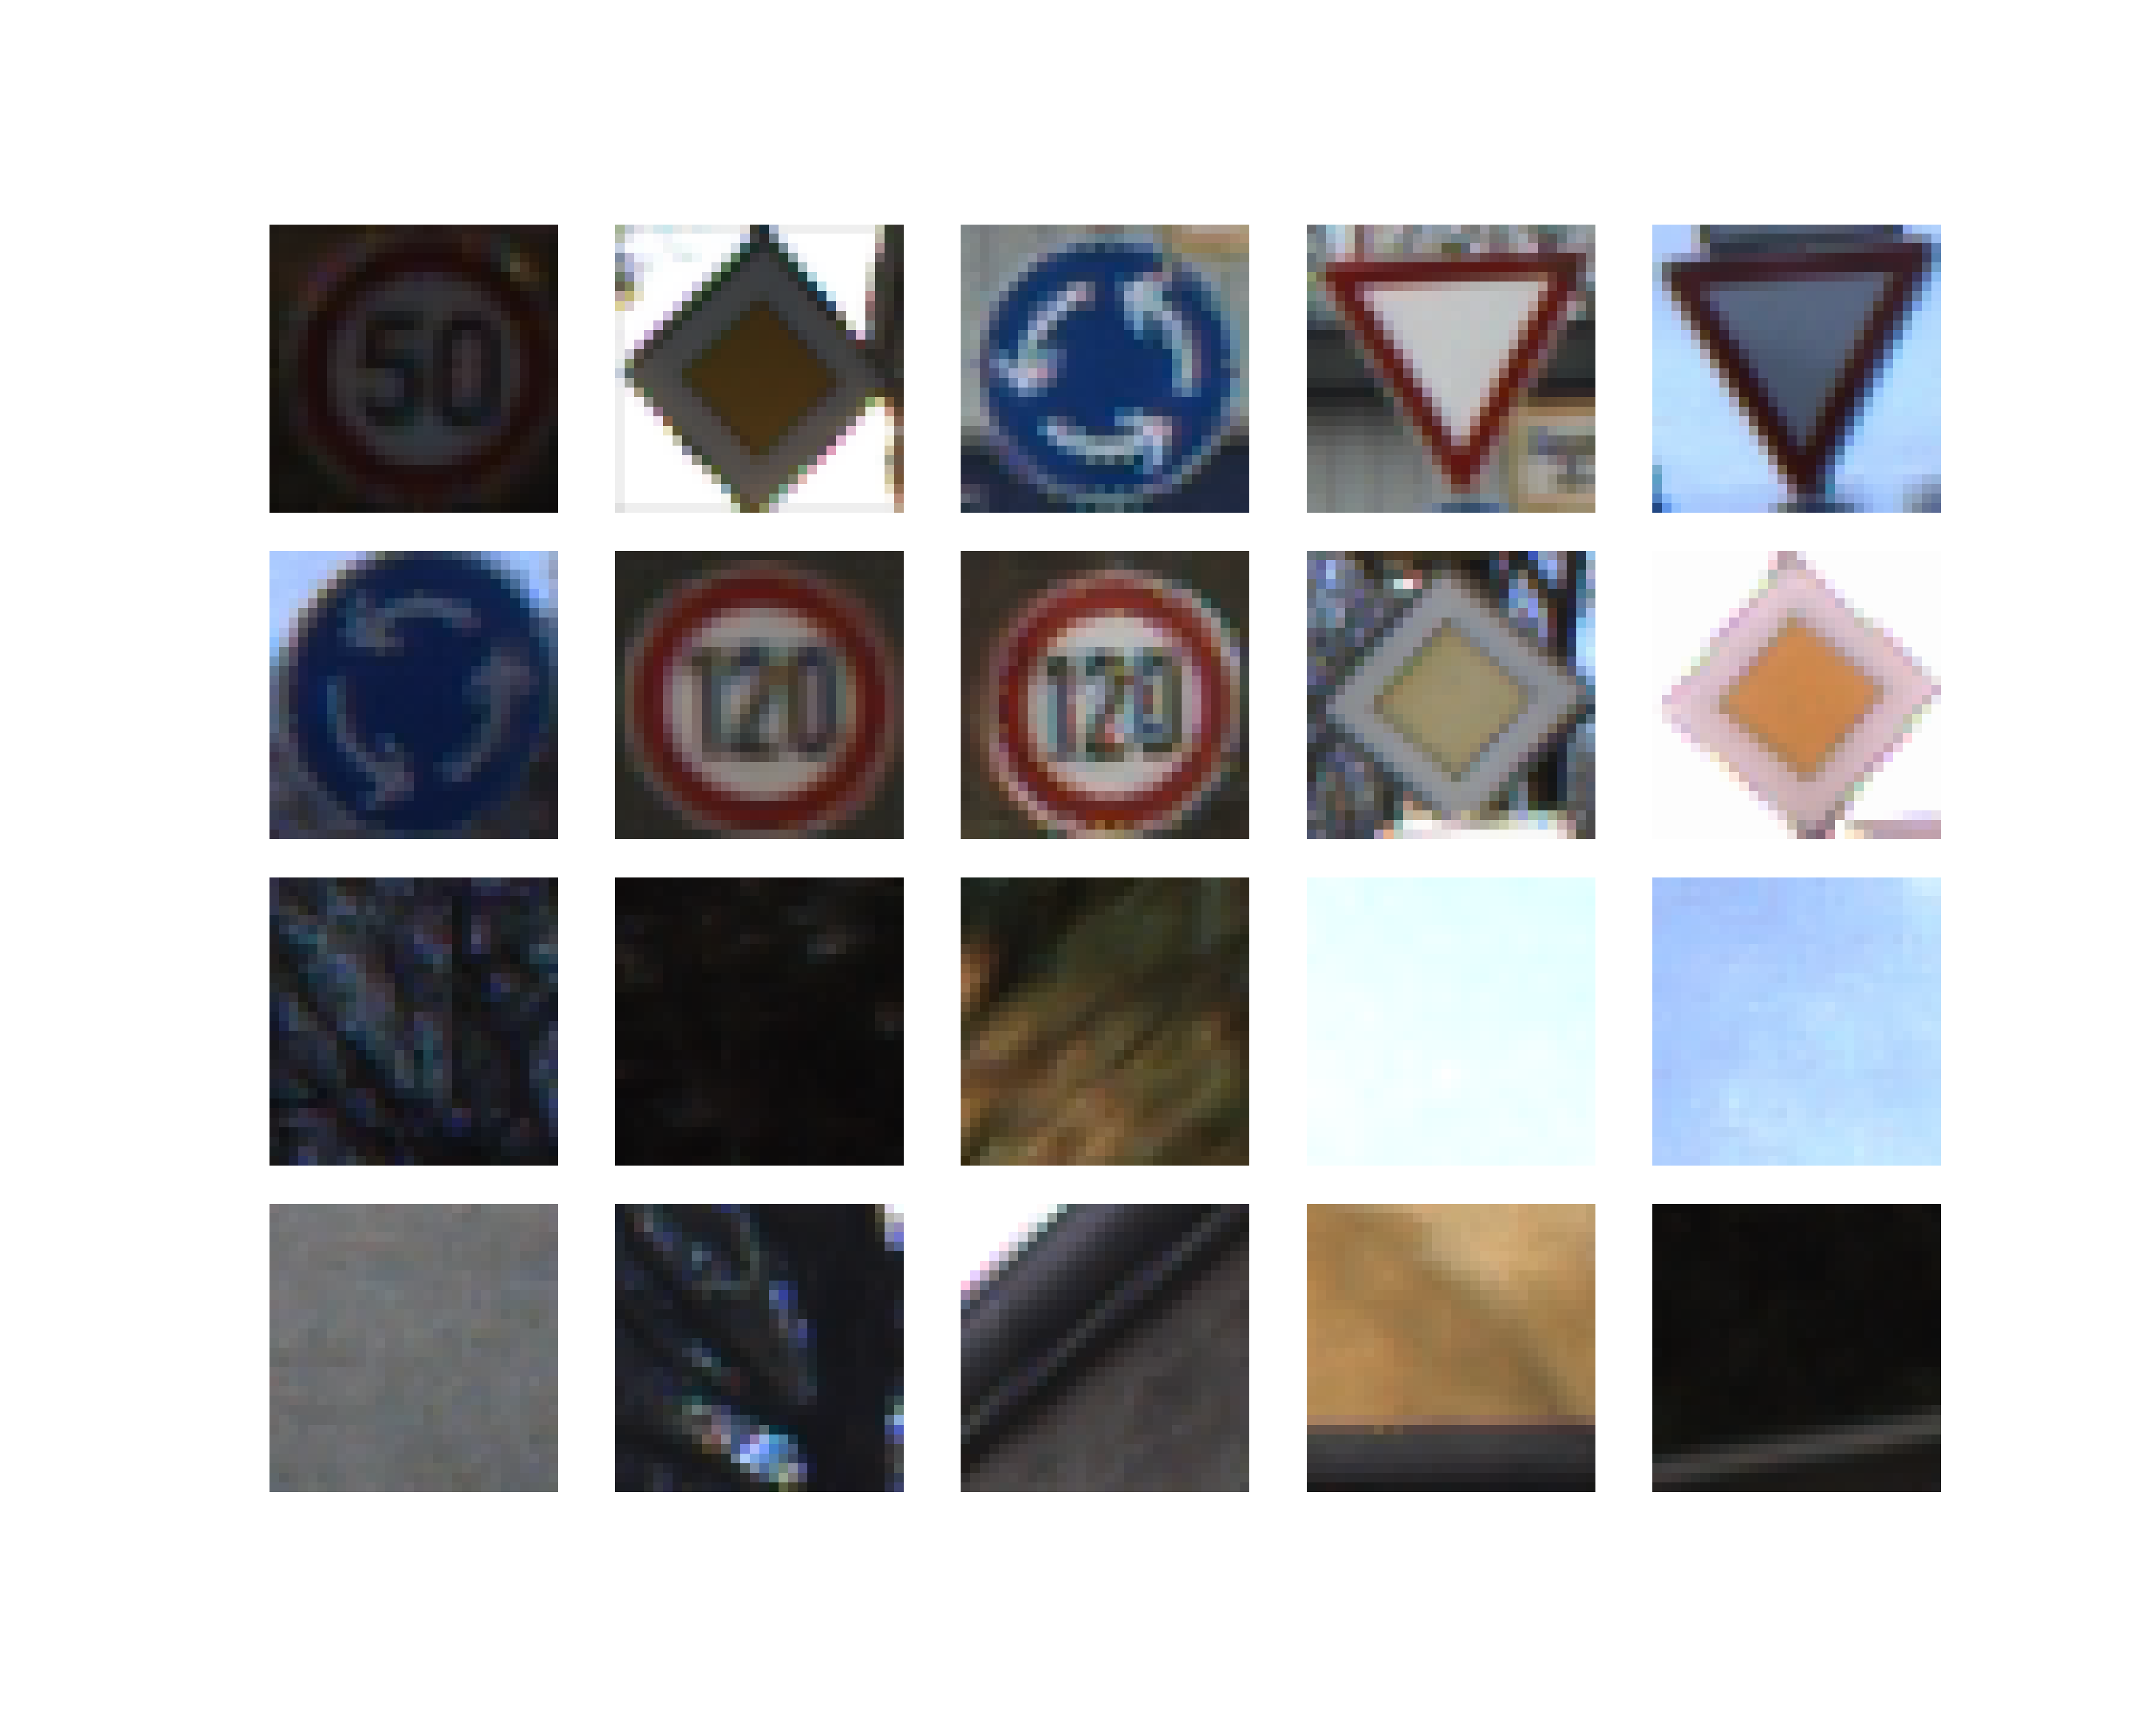
\includegraphics[width=0.6\linewidth]{pos_neg_patches.png}
  \caption{The first and second row show positive patches containing traffic signs, the third and fourth row show negative patches without a traffic sign contained. The size of all patches is $30 \times 30$ pixels.}
  \label{fig:posnegpatch}
\end{figure}


\subsection{Feature extraction using HOG}

\subsubsection{Theory HOG}
The \textbf{H}istogram of \textbf{O}riented \textbf{G}radients (HOG) is a feature descriptor widely used in the context of object detection. This method basically summarizes gradient orientations in localized sections of an image by performing the following five steps \cite{Dalal}: 

\begin{enumerate}
	\item Global image normalization using gamma compression: thereby one can compensate for variations in illumination or local shadowing effects.
	\item Computation of first order image gradients.
	\item Computation of gradient histograms: in so-called cells of predefined size (e.g. $5 \times 5$ pixels) gradient orientations over all pixels in the cell are accumulated in a histogram. 
	\item Normalization across blocks: as gradient strength must be locally normalized cells are grouped together into so-called blocks, on which normalization is performed. Possible methods for block normalization are, for instance, the L1-norm or the L2-norm.
	\item Collection of HOG descriptors from all cells into a combined feature vector. 
\end{enumerate}

\subsubsection{Application}
We used the HOG implementation from scikit-image \cite{scikithog}. As proposed by Houben \textit{et al.} who performed a similar approach, we considered 8 gradient orientations, used cells of size $5 \times 5$ pixels and a block size of $2 \times 2$ cells \cite{Houben-IJCNN-2013}. As block normalization method we chose the L2 normalization.
The final training set used to train the SVM is then constructed from the HOG features of the positive and negative patches. 

\subsection{Classification using SVM}
\subsubsection{Theory SVM}
A support vector machine is a well established supervised classification and regression method. Given a set of labeled training examples from two classes - positive and negative - a SVM training algorithm creates a model that can assign new examples to one category or the other. Formally, a SVM constructs a hyperplane by maximizing the margin between positive and negative data points (see Figure \ref{fig:svm}).  

\begin{figure}[H]
\centering
  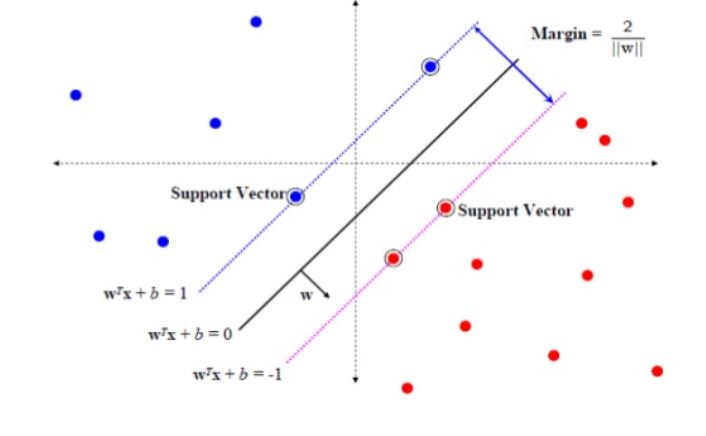
\includegraphics[width=0.7\linewidth]{svm.jpg}
  \caption{A Support Vector Machine tries to maximize the margin between positive and negative data points. Source: \url{https://www.slideshare.net/kambliruta/event-classification-prediction-using-support-vector-machine}}
  \label{fig:svm}
\end{figure}

\subsubsection{Training}
We used the SVM implementation provided by sklearn \cite{sklearnsvm} with the default values except for the kernel which we chose to be linear. With the intention to improve performance of the SVM as well as to obtain a sufficiently large training set, we additionally included a step of Hard Negative Mining (HNM). 
Therefore, the SVM is first trained with the previously constructed training set. Then, for every image and possible scale of the images dedicated for training, that contain no traffic sign, we apply the sliding window technique. At each window we compute the HOG descriptors and employ the pre-trained SVM. Each falsely detected patch is taken and explicitly added as a negative example to the training set. Finally, the SVM is retrained using the enlarged training set.
In the results section we compare the outcome with and without Hard Negative Mining based on the achieved training / test accuracies. \\
We expect a significant improvement when training with Hard Negative Mining as we obtain more variety in the negative training samples especially by using different scales of the images. Here we used $\sqrt(2)^i$ with $i = 0,...,-5$ as scale factor to obtain an image pyramid with $6$ layers including the original image. By the use of an image pyramid for Hard Negative Mining we can capture larger structures which might get confused easily with a traffic sign and explicitly learn the classifier to recognize them as negative examples.   

\subsubsection{Detection}
For detection of traffic signs in a given image we slide a window of size $30 \times 30$ pixels across the image at different scales - here we also used an image pyramid with  scale factor $\sqrt(2)^i$ where $i = 0,...,-5$ - and obtain a prediction for every image section from the SVM. If the thereby received regions possibly showing a traffic sign are obtained from another than the original scale of the image these are back computed to the original image's size. As a result we finally obtain a list of predicted bounding boxes relating to the original input image.

\subsubsection{Performance Measure} \label{ssec:perf}
For a quantitative measure of the detection performance each predicted bounding box $P$ is compared against every ground truth bounding box $G$ by means of the Jaccard similarity, which is defined as the intersection over union of the two bounding boxes: 
\begin{align*}
	S(P,G) = \frac{|P \cap G|}{|P \cup G|}
\end{align*}
If $S(P,G) \geq 0.5$ for any predicted bounding box $P$, the ground truth sign $G$ is considered as detected. In the end, we record the fraction of detected ground truth signs in all images. \\
In addition, a measure for the amount signs detected erroneously - i.e. the false positive rate - is needed. Therefore, we assess the fraction of predicted bounding boxes that have zero overlap with any of the ground truth bounding boxes. 

\pagebreak
\section{Second Approach: RNN \small{(Marvin)}}

\pagebreak
\section{Results}
\subsection{First Approach \small{(Daniela)}}

The average detection performance on 30 randomly chosen images from the training respectively test set is reported in Table \ref{tab:perf}. Contrary to our expectations the accuracy seems to decrease when training the SVM with HNM. However, when having a look at the bounding box predictions of the SVM trained with respectively without HNM, which are presented in Figure \ref{fig:compar}, one can see that Hard Negative Mining significantly lowers the false positive rate. On the left image both ground truth bounding boxes are detected, however there is a large amount of false positives. In the right image the second ground truth bounding box is not found, but the false positive rate is much lower. Unfortunately the amount of false positives is not taken into account by the performance measure we used. Thus we nevertheless assess Hard Negative Mining as an improvement and keep applying it when training our classifier.

\begin{table}[H]
\centering
\caption{Detection performance and false positive rate on the train respectively test set obtained with and without HNM. For training and detection a sliding window of $30 \times 30$ pixels was used. The window's step size was $10$ pixels for training and $5$ pixels for detection.}
  \begin{tabular}{l| c c c c}
  	  & 
      \multicolumn{2}{c}{\textbf{train acc}} &
      \multicolumn{2}{c}{\textbf{test acc}} \\
    & performance & false positives & performance & false positives \\ \toprule
    \textbf{w/o HNM} & 95.0\% & 84,91\% & 99,17\% & 93,71\% \\
    \textbf{HNM} & 86,39\% & 11.6\% & 91,67\% & 11.6\% \\
  \end{tabular}
\end{table}



\begin{table}[H]
\centering
\caption{Detection performance and false positive rate on the train respectively test set obtained with and without HNM. For training and detection a sliding window of $30 \times 30$ pixels was used. The window's step size was $10$ pixels for training and $5$ pixels for detection.}
\label{tab:perf}
\small
\begin{tabular}{ l | r r }
  &  train acc & test acc \\ \toprule
  w/o HNM & 93.05,95.0 \% & 89.17, 99.17 \% \\
  w HNM & 85.56, 86,39 \% & 79.17,91,67 \% \\
\end{tabular}
\end{table}

\begin{figure}[H]
\begin{minipage}{0.48\textwidth}
\centering
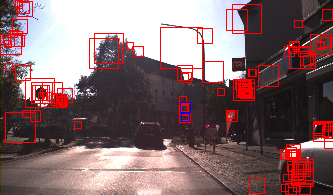
\includegraphics[width=\linewidth]{train102_wo_hn_prediction.png}
\end{minipage}
\hfill
\begin{minipage}{0.48\textwidth}
\centering
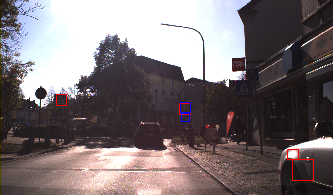
\includegraphics[width=\linewidth]{train102_predboxes2.png}
\end{minipage}
\caption{Bounding box prediction for the same image once using a SVM trained without HNM (left) and once trained with HNM (right). Ground truth bounding boxes are indicated in blue and predicted bounding boxes in red.}\label{fig:compar}
\end{figure}

In Figure \ref{fig:train_img_bbox} some training images are shown in which the ground truth bounding boxes are indicated in blue while the predicted bounding boxes are drawn in red. The respective detection performances are noted below. Almost all traffic signs - if present - are detected and there are only few false positive predictions. Especially interesting is the image in the upper middle: while the construction site sign is not detected possibly due to the poor lighting conditions, the hexagonal light spot in the upper left corner is recognized as a traffic sign instead. 

%% Result images test set
\begin{figure}[H]
\begin{minipage}{0.3\textwidth}
\centering
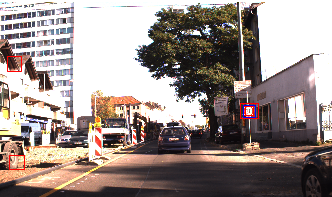
\includegraphics[width=\linewidth]{train0_predboxes2.png}
\small{(100\%)}
\end{minipage}
\hfill
\begin{minipage}{0.3\textwidth}
\centering
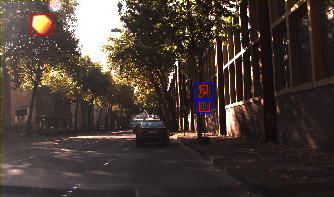
\includegraphics[width=\linewidth]{train23_predboxes2.png}
\small{(50\%)}
\end{minipage}
\hfill
\begin{minipage}{0.3\textwidth}
\centering
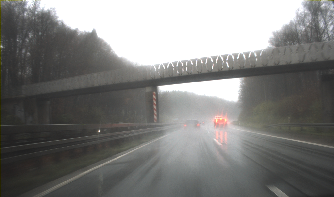
\includegraphics[width=\linewidth]{train212_predboxes2.png}
\small{(100\%)}
\end{minipage}

\begin{minipage}{0.3\textwidth}
\centering
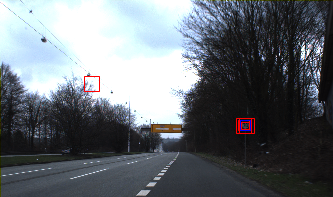
\includegraphics[width=\linewidth]{train407_predboxes2.png}
\small{(100\%)}
\end{minipage}
\hfill
\begin{minipage}{0.3\textwidth}
\centering
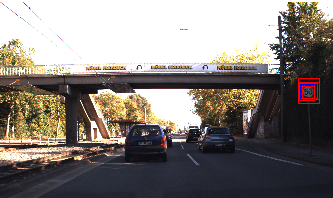
\includegraphics[width=\linewidth]{train599_predboxes2.png}
\small{(100\%)}
\end{minipage}
\hfill
\begin{minipage}{0.3\textwidth}
\centering
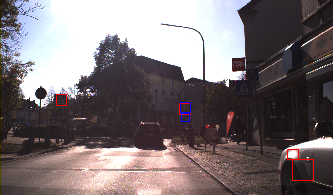
\includegraphics[width=\linewidth]{train102_predboxes2.png}
\small{(50\%)}
\end{minipage}
\caption{Images from the training set with ground truth bounding boxes in blue and predicted bounding boxes in red. Prediction accuracy in percentage according to the prediction measure explained in section \ref{ssec:perf} is given below each image.}
\label{fig:train_img_bbox}
\end{figure}

Figure \ref{fig:test_img_bbox} shows images from the test set along with ground truth and predicted bounding boxes. One can see that almost all traffic signs are detected as it was the case for the training images except for the rightmost sign in the upper middle image and the lower right image. If there is no traffic sign at all like in case of the bottom middle image, the algorithm does also recognize that correctly. However, the upper right and lower left image show that there are still sometimes false positives, which is not punished by our performance measure. Possibly the number of false positives can be reduced if another step of Hard Negative Mining is included.

%% Result images test set
\begin{figure}[H]
\begin{minipage}{0.3\textwidth}
\centering
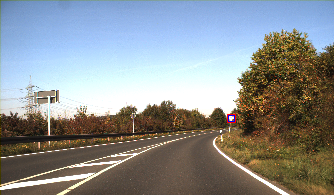
\includegraphics[width=\linewidth]{test2_wb_predboxes2.png}
\small{(100\%)}
\end{minipage}
\hfill
\begin{minipage}{0.3\textwidth}
\centering
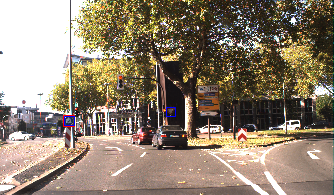
\includegraphics[width=\linewidth]{test14_wb_predboxes2.png}
\small{(50\%)}
\end{minipage}
\hfill
\begin{minipage}{0.3\textwidth}
\centering
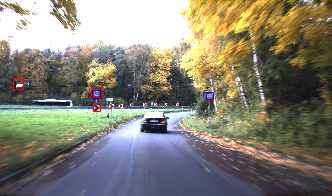
\includegraphics[width=\linewidth]{test44_wb_predboxes2.png}
\small{(100\%)}
\end{minipage}

\begin{minipage}{0.3\textwidth}
\centering
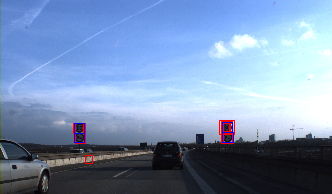
\includegraphics[width=\linewidth]{test144_wb_predboxes2.png}
\small{(100\%)}
\end{minipage}
\hfill
\begin{minipage}{0.3\textwidth}
\centering
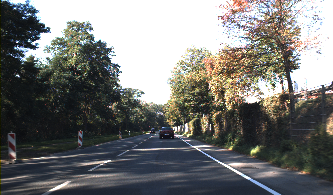
\includegraphics[width=\linewidth]{test200_wb_predboxes2.png}
\small{(100\%)}
\end{minipage}
\hfill
\begin{minipage}{0.3\textwidth}
\centering
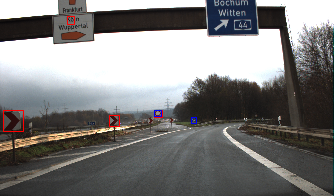
\includegraphics[width=\linewidth]{test100_wb_predboxes2.png}
\small{(50\%)}
\end{minipage}
\caption{Images from the test set with ground truth bounding boxes in blue and predicted bounding boxes in red. Prediction accuracy in percentage according to the prediction measure explained in section \ref{ssec:perf} is given below each image.}
\label{fig:test_img_bbox}
\end{figure}

Finally, we wanted to observe how the sliding window's step size during detection affects the performance. Figure \ref{fig:step_perf} plots the resulting performance against the detection step size. Already with very few data points it becomes clear that the detection step size is very critical to the success of traffic sign detection. 

\begin{figure}[H]
\centering
  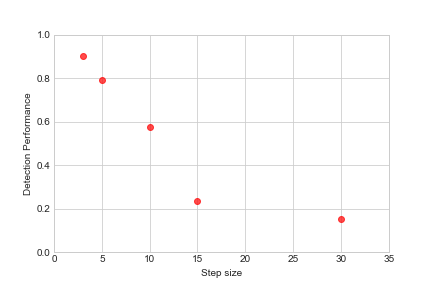
\includegraphics[width=0.5\linewidth]{step_performance}
  \caption{Detection performance on 30 randomly chosen images from the training set versus the step size of the sliding window used for detection.}}
  \label{fig:step_perf}
\end{figure}


\subsection{Second Approach \small{(Marvin)}}

\pagebreak
\section{Discussion}
To sum up the first approach, one can say that HOG features learned by a SVM are very well suited to detect traffic signs in color images. By the use of Hard Negative Mining the false positive rate can be lowered significantly, however, one looses some accuracy at the same time. Generally, the approach is very sensitive to the setting of the hyperparameters especially towards the step size of the sliding window for detection. The smaller the step size the better the detection performance - at the price to a much higher computational effort. It could thus be an improvement to use region of interest extraction instead of a sliding window, like for instance selective search, which was basically done in the second approach by the R-CNN. 


\begin{itemize}
	\item je nachdem welches measure genommen werden falsch positive halt ignoriert...außerdem könnte man IOU>=0.5 auch schon nehmen.
\end{itemize}


\section{Appendix}
\subsection{Appendix A}
0 = speed limit 20 (prohibitory) \\
1 = speed limit 30 (prohibitory) \\
2 = speed limit 50 (prohibitory)\\
3 = speed limit 60 (prohibitory)\\
4 = speed limit 70 (prohibitory)\\
5 = speed limit 80 (prohibitory)\\
6 = restriction ends 80 (other)\\
7 = speed limit 100 (prohibitory)\\
8 = speed limit 120 (prohibitory)\\
9 = no overtaking (prohibitory)\\
10 = no overtaking (trucks) (prohibitory)\\
11 = priority at next intersection (danger)\\
12 = priority road (other)\\
13 = give way (other)\\
14 = stop (other)\\
15 = no traffic both ways (prohibitory)\\
16 = no trucks (prohibitory)\\
17 = no entry (other)\\
18 = danger (danger)\\
19 = bend left (danger)\\
20 = bend right (danger)\\
21 = bend (danger)\\
22 = uneven road (danger)\\
23 = slippery road (danger)\\
24 = road narrows (danger)\\
25 = construction (danger)\\
26 = traffic signal (danger)\\
27 = pedestrian crossing (danger)\\
28 = school crossing (danger)\\
29 = cycles crossing (danger)\\
30 = snow (danger)\\
31 = animals (danger)\\
32 = restriction ends (other)\\
33 = go right (mandatory)\\
34 = go left (mandatory)\\
35 = go straight (mandatory)\\
36 = go right or straight (mandatory)\\
37 = go left or straight (mandatory)\\
38 = keep right (mandatory)\\
39 = keep left (mandatory)\\
40 = roundabout (mandatory)\\
41 = restriction ends (overtaking) (other)\\
42 = restriction ends (overtaking (trucks)) (other)\\

\subsection{Appendix B: Requirements}
As programming language python 3.6 was used. The following modules are needed to execute the code:
\begin{itemize}
	\item os
	\item numpy
	\item math
	\item matplotlib
	\item imageio
	\item random
	\item seaborn
	\item sklearn
	\item skimage
	\item scipy
	\item pandas
	\item selectivesearch
	\item torch
\end{itemize}

% ----------------------------------------------------------------------------------------------------------
% Literatur
% ----------------------------------------------------------------------------------------------------------

\renewcommand\refname{References}
\bibliographystyle{acm}
\bibliography{bibo}
\pagebreak


\end{document}
